\chapter{Grundlagen}
\thispagestyle{standard}
\pagestyle{standard}
\renewcommand{\footrulewidth}{0.4pt}
\lfoot{\small Refik Kerimi}

Wie in Kapitel \ref{chap:Einleitung} beschrieben, hat der stetige Zuwachs von Smart Phones zum Umdenken bei der Planung und bei der Entwicklung von \acl{Web-App}s geführt.
Zu Beginn jedes Projektes steht die Entscheidung an, welche Technologien und Tools zur Entwicklung verwendet werden sollen um die bestmöglichen Ergebnisse zu erhalten.
Wenn die falschen Methoden gewählt werden, kann das zu gravierenden Fehlern in der Applikation führen, die erst mit Fortdauer der produktiven Verwendung ersichtlich werden. 
Die Frage ist, ob man sich für eine Anwendung, die auf das Betriebssystem zugeschnitten ist, oder doch für eine plattformübergreifende Webanwendung entscheidet. Beide Methoden haben Vorteile und Nachteile und werden im Zuge dieser Arbeit betrachtet. Den Kern der Arbeit stellt die von Google entwickelte \acs{PWA}  da. \\Die \acs{PWA}s sollen den Spagat zwischen diesen beiden Anwendungen schaffen. Eventuell könnte diese neue Form der Appentwicklung die traditionellen Technologien gar zur Gänze ablösen.
Der Trend der letzten Jahre geht in Richtung der mobilen Nutzung und da ist das Smart Phone klar wie, in Abbildung \ref{fig:Smartphonenutzung} dargestellt, voran  \cite{Geraetenutzung} \cite{PWA}.  


\begin{figure}[h]
	\centering
	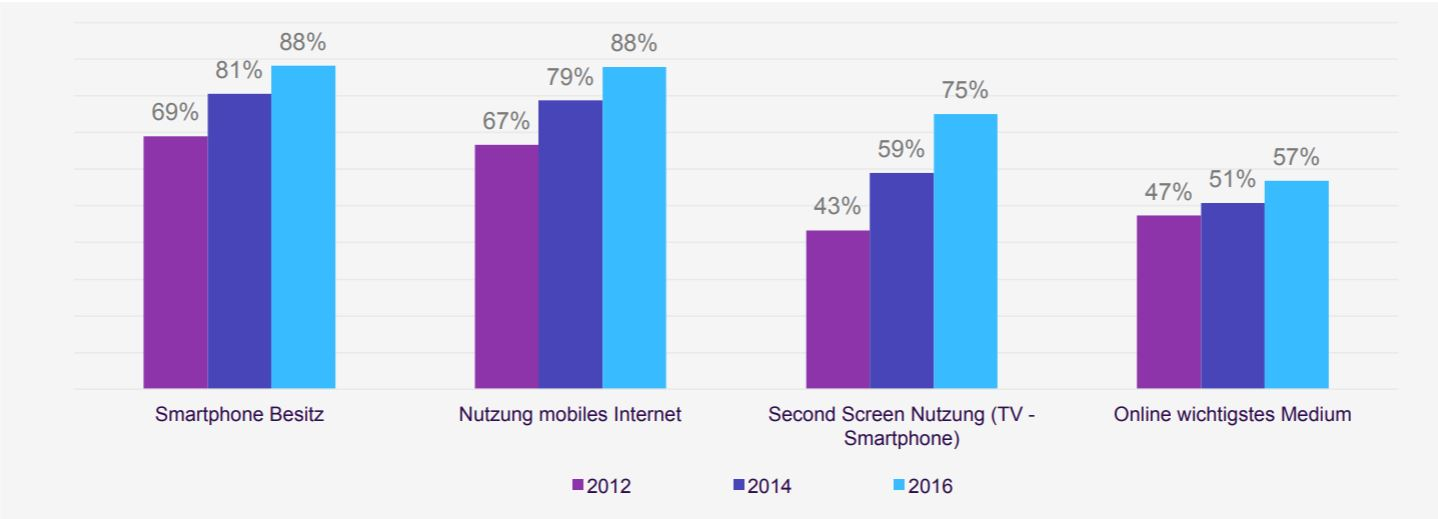
\includegraphics[width=11cm]{BilderAllgemein/SmartPhoneNutzung}\medskip
	\caption{Smartphonenutzung Österreich 2016 \cite{Geraetenutzung}}
	\label{fig:Smartphonenutzung}
\end{figure}

\newpage
\section{Geschichte Softwareentwicklung}
Im Laufe der Jahre wurde verschiedenste Software entwickelt, die mehr oder weniger nützlich für unseren Alltag war.
Der Begriff Software wurde 1958 vom US-amerikanischen Statistiker John W. Turkey eingeführt.
Zu Beginn bildeten Software und Hardware eine Einheit. Erst nach der Entscheidung durch die US Regierung, dass IBM die Hardware und die Software separat verrechnen sollte, wurden sie getrennt. \\
Die Software bildet das Gehirn eines Computers.
Es folgte in den 1970er Jahren die Gründung von rein softwareorientierten Firmen wie Microsoft oder SAP \cite{Microsoft} \cite{SAP}. 

\section{Native Apps}\label{chap:Native Apps}
Native Apps sind speziell für eine Plattform angepasste Anwendungen. 
Diese werden für ein bestimmtes Betriebssystem konzipiert und haben in der Regel Zugriff auf alle Ressourcen eines Gerätes .
Hauptsächlich werden zur Programmierung für mobile Geräte die Hochsprachen Java (Android) und Swift (IOS) verwendet. Native Apps können in App Stores heruntergeladen  werden. \\Die bekanntesten sind Apple Store und Google Play \cite{NativeApp} \cite{Hochsprachen}.

\section{Web App}\label{chap:Webapplikationen}
Im Gegensatz zu den nativen Apps sind \acl{Web-App}s (\acs{Web-App}) speziell programmierte Webseiten .
\acs{Web-App} funktionieren nach dem Server-Client Prinzip und werden vom Browser aufgerufen. In der Regel werden \acs{Web-App}s auf der Basis von \acs{JS}, \acs{CSS} und \acs{HTML}5 entwickelt. Die Verarbeitung erfolgt auf dem Webserver oder auf der Cloud. 
Der größte Vorteil ist sicherlich der unkomplizierte Zugang im Gegensatz zu den Native App.
Durch die Einführung von Responsive Frameworks wie z.B.: Bootstrap, SemantikUI oder Foundation um nur die bekanntesten zu nennen, wurde die Webentwicklung vielseitiger in der Verwendung. Durch diese Technologien können viele Bildschirmgrößen mit wenig Aufwand abgedeckt werden \cite{Hochsprachen} \cite{WebApps} \cite{CSS}. 

\section{Hybrid App}
Hybrid Apps verbinden die Eigenschaften der in Kapitel \ref{chap:Native Apps} und \ref{chap:Webapplikationen} genannten Technologien. Zum einen verwenden sie die webbasierende Client-Server Technologie, zum anderen kann man mit einer Hybrid App auf Gerätefunktionen wie Kamera und Kalender zugreifen \cite{HybridApps}. 

\section{Progressive Web App}\label{chap:ProgressiveWebapplikationen}
\acl{PWA}s sind im Grunde eine Weiterentwicklung einer \acs{Web-App}s. Diese Technologie der Webentwicklung wird durch die schneller wachsende Welt der Webanwendungen immer wichtiger. 
Dem User wird das Gefühl gegeben, mit einer nativen App zu arbeiten. Das Herausragende dabei ist, im Gegensatz zu einer Hybrid App, dass jede bestehende \acs{Web-App} in eine \acs{PWA} umgebaut werden kann.
Durch Hinzufügen einer Manifest Datei und eines Service Worker werden Features erweitert, die es ermöglichen offline zu arbeiten oder das Icon der App auf den Desktop oder Home-Bildschirm zu speichern \cite{PWA} \cite{PWAAdjectives}.\\ \\
Google definiert die \acs{PWA} wie folgt :
\begin{itemize}
    \item  \textbf{Progressive} - funktioniert für alle User unabhängig vom Browser
	\item  \textbf{Responsive} - passt sich jedem Gerät an	
	\item  \textbf{Verbindungsunabhängig} - funktioniert auch bei schlechtem oder gar keinem Internetzugang
	\item  \textbf{App-like} - fühlt sich an wie eine Native App
	\item  \textbf{Aktuell} - durch die Wartung des Service Workers immer auf dem aktuellsten Stand
	\item  \textbf{Sicher} - wird nur über HTTPS bereitgestellt
	\item  \textbf{Erkennbar} - erkennbar dank das W3C Manifest durch Suchmaschinen
	\item  \textbf{Wiedereinschaltbar} - wird durch die Funktion Push Notfication erreicht
	\item  \textbf{Installierbar} - ermöglicht das Hinzufügen auf dem Startbildschirm
\end{itemize}. 


